\documentclass[11pt,twoside]{scrbook}

\usepackage{a4}
\usepackage{times}
\usepackage{graphicx}
\usepackage{listings}
\usepackage[english,iso]{isodate}
\usepackage[utf8x]{inputenc}
\usepackage{tocloft}
\usepackage{pdfpages}
%\usepackage{verbatimfiles}

%\usepackage[outline,light]{draftcopy}

\usepackage[pdfauthor={Stefan Schmidt},pdftitle={Delay Tolerant Networking on
Embedded Linux Hardware},pdfkeywords={802.15.4, LowPAN, LR-WPAN, DTN, IBR-DTN,
linux, Imote2}]{hyperref}

% We want the caption position of listings at the bottom
\lstset{captionpos=b}

% So wird's gemacht, wenn in den Text EPS-Bilder eingefuegt werden sollen!
% \begin{figure}[htb]
% \centerline{\includegraphics[width=\textwidth]{bild1.eps}}
% \caption{\label{bild1}Title of the picture.}
% \end{figure}

\begin{document}

%Deckblatt erzeugen
\thispagestyle{headings}
\title{Delay Tolerant Networking on Embedded Linux Hardware}
\author{Stefan Schmidt}

\maketitle
\setcounter{page}{1}
\pagenumbering{roman}

\thispagestyle{headings}
\begin{titlepage}
	\let\footnotesize\small
	\let\footnoterule\relax
	\null
	\vfil
	\vskip 60pt
	\begin{center}
		{\LARGE
			{\Large Technische Universität Braunschweig}\\
			Institut für Betriebssysteme und
				Rechnerverbund\\[2cm]
			{\Large Studienarbeit}\\ [2cm]
			Delay Tolerant Networking on Embedded Linux Hardware
			\par}%
		\vskip 6em
		{\large \lineskip .75em
		\begin{tabular}[t]{c}
			{\Large von}\\[.5em]
			{\Large cand. inform.\ Stefan Schmidt}\\[7em]
			{\bf Aufgabenstellung und Betreuung:}\\[.5em]
			Prof.\ Dr.\ L.\ Wolf.  und
			Dipl.-Inform.\ W.\ Pöttner\\
		\end{tabular}
		\par}%
		\vfill
		{\large
			Braunschweig, den \today
			\par}%
	\end{center}
	\par
	% thanks
	\vfil
	\null
\end{titlepage}

~\newpage

% Erklaerung
\vspace*{7cm}
\centerline{\bf Erklärung}

\vspace*{1cm}
Ich versichere, die vorliegende Arbeit selbstständig und nur unter Benutzung
der angegebenen Hilfsmittel angefertigt zu haben.

\vspace*{3cm}
%\centerline{Braunschweig, den \today \hfil \hfil Unterschrift}
Braunschweig, den \today

\pagestyle{headings}
\cleardoublepage

\centerline{\bf Abstract}

This example abstract is indeed very abstract.

\cleardoublepage


\includepdf[pages={1,2}]{../ibr_aufgabenstellung.pdf}

\cleardoublepage
\tableofcontents
\cleardoublepage
\listoffigures
%\cleardoublepage
\listoftables
%\cleardoublepage

%\parindent=0pt                   % erzeugt bei einem Absatz eine
%\parskip=6pt plus 3pt            % Leerzeile (kein Einruecken)

\setcounter{page}{0}

\pagestyle{headings}
\pagenumbering{arabic}

\chapter{Introduction}
While approaching a more and more ubiquitous network experience where we are
connected to different personal area networks (PAN) or even the global internet
around the clock two problems become more important. One problem is the power
consumption of devices which make the ubiquity possible. In contrast to other
computing devices we want them to be well hidden and unintrusive. Changing
batteries or having power cables around is not a real option for them. On the
other hand wireless communication protocols with IEEE 802.11 \cite{ieee80211} as the
leading option are a good choice for mobile devices like notebooks or
smartphones but are still to power hungry for small ubiquitous devices.
With IEEE 802.15.4 \cite{ieee802154} a new protocol was designed for exactly such
small, power constraint devices. We will use it in our research and have some
more information about it prepared in section~\ref{intro802154}.

The second problem are network connection disruptions - be it due to movement or
the other changes. The most widely used protocol family with IP, UDP, TCP is not
designed to cope with disrupted networks. They need an established physical connection
to work as expected. If this is not the case the packets may be just lost
as in case of UDP or have to be re-transmitted. This re-transmission could be
problematic if the network connection is unavailable more often then available.
For such scenarios delay tolerant networking was designed to send the
packets, perhaps over several hops, to the destination without needing to
establish a channel between source and destination. In~\ref{introdtn} we give a
short introduction to DTN before describing the IBR-DTN implementation in chapter
\ref{ibr-dtn} and our convergence layer in chapter \ref{802154layer}.

\section{IEEE 802.15.4}
\label{intro802154}
Driven by an IEEE working group the IEEE 802.15.4 standard provides the physical and
media access control layer for so called low-rate wireless personal area network
(LR-WPAN). The emphasis is on low cost devices for communication without
infrastructure over small distances. The offered transfer rate can be up to 250 kbps.
The standard specifies three possible frequency bands to operate in. 16 channels
in the 2450 MZz band, 10 channels in the 915 MHz band and one channel in the 868
MHz band. The usage of some may be restricted in different countries but 2450 MHz
band is available worldwide.
Other features of IEEE 802.15.4 includes collision avoidance through CSMA/CA, built
in support for secure communication through cryptography, power management through
link quality control and energy detection as well as acknowledgements,
retransmissions and reserved time slots for real-time operations.

As already described the standard only covers the two lowest layer of a
protocol stack. Supplementing it to a fully functional networking stack is the aim
of different other specifications as shown in figure~\ref{fig:802154layer}. The
most widely know is be ZigBee. With 6LowPAN there is also work underway to combine
LR-WPAN with standard internet protocols like IPv6.

Specified for an infrastructure-less network the topologies may be star or
Peer-to-Peer based as well a combination of both. Figure \ref{fig:802154topologies}
shows examples for these topologies. Two different device types are allowed:
full-function device (FFD) and
reduced-function device (RFD). The RFD is a very simple device which can only
connect to one FFD at a time. Therefore it can only act as a leaf in all
described topologies. In contrast, the FFD is able to act as a coordinator to
create a new PAN and relay messages to other nodes. At least one coordinator
is needed in every network. It creates the network and assigns addresses to
associating nodes. These assigned addresses are short addresses with only 16 bit
and only unique withing the PAN. Additionally every node has a long address with
64 bit unique worldwide. One thing to keep in mind is that routing is not
covered by the standard. To relay messages over multiple hops the supplementing
upper layers need to take care of this.

\begin{figure}
  \begin{center}
    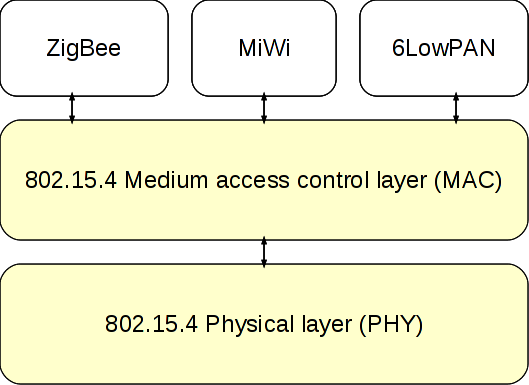
\includegraphics[height=6cm]{images/802154layer}
    \caption{IEEE 802.15.4 lower layers with optional upper layers}
        \label{fig:802154layer}
  \end{center}
\end{figure}

\begin{figure}
  \begin{center}
    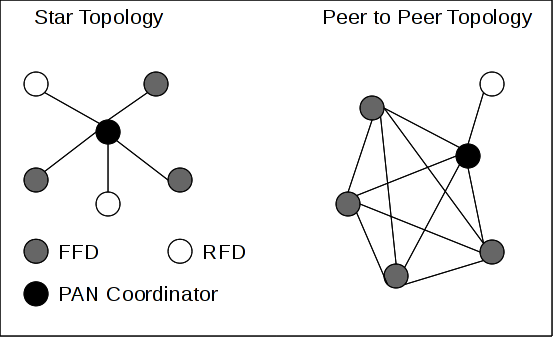
\includegraphics[height=6cm]{images/802154topology}
    \caption{IEEE 802.15.4 network topologies}
        \label{fig:802154topologies}
  \end{center}
\end{figure}

\section{DTN}
\label{introdtn}
The need for communication between nodes without continuous network
connectivity is what DTN seeks to address. Most modern routing protocols only
send out the payload once a complete route to the destination has been established.
A communication over such an approach is only possible if source and destination
are connected to a network long enough to establish a route between them,
transfer the data and possibly acknowledge the transfer.

DTN in contrast uses a store and forward approach which sends out the data
together with the destination address. The bundle protocol in
\cite{RFC5050} was specified for this. One approach to maximize the probability
of a successful delivered message would be to send out multiple copies of the
same message, maybe to different hops. Such an approach obviously increases the
network and storage load and may not be useful for constrained devices like
sensor nodes.

The bundle protocol specifies an overlay network which interacts with the lower
layers over convergence layers. The lower layers are not bound to be IP
based even if that is the one widely used. In this thesis we describe the usage
of the DTN implementation IBR-DTN over an IEEE 802.15.4 radio link on a Linux
based system.


\chapter{Imote2 Hardware}
For this thesis the Imote2~\cite{imote2} hardware platform was used as it allowed us to use
standard Linux environment while acting like a wireless sensor network node to
the outside. The Imote2 platform
consists of different pluggable boards to extend it with sensors or multimedia
capabilities. For our work we only used the Imote2 Processor Radio Board
(IPR2400) and the Interface Board (IIB2400) for serial console access and JTAG.

While other sensor nodes are tightly constrained regarding their computing power
and storage, the Imote2 is based on a powerful XScale CPU and equipped with 32
MByte of SDRAM as well as flash storage. This comes of course with a higher power
consumption cost compared to microcontroller based sensor nodes like the T-Mote
Sky~\footnote{http://www.snm.ethz.ch/Projects/TmoteSky}. On the other hand
exactly these components are allowing us to run a full
Linux and DTN system on the node and allow comfortable development and rapid
prototyping.

\section{Processor Radio Board}
As the name suggests this is the base board all other boards rely on. It holds
the PXA271 XScale ARM System on a Chip with a CPU frequency from 13 to 416 MHz
as well as the SDRAM and flash storage. If configured for a frequency from 13
to 104 MHz the CPU can be used in a low power mode on a low voltage level
(0.85V). This was not done during this work, but would be an interesting target
for later deployment. Instead we used the CPU at the full frequency of 416 MHz
during development and evaluation.

The PXA271 offers a wide range of peripheral components already built in. The
connectors for these are available on the basic and advanced connectors on the
board. Examples are USB host and client, SDIO, UART, AC97 and I2S audio
interfaces, I2C, SPI and GPIOs. USB client is already routed to a mini USB
connector on the board. This can be used to access the system and supply power
over USB.

Figure~\ref{fig:imote2top} is a top view of the IPR2400 showing the USB client plug,
the board connectors and the IEEE 802.15.4 radio transceiver with the onboard
antenna. We go into more details about it in section~\ref{cc2420}.

\begin{figure}
  \begin{center}
    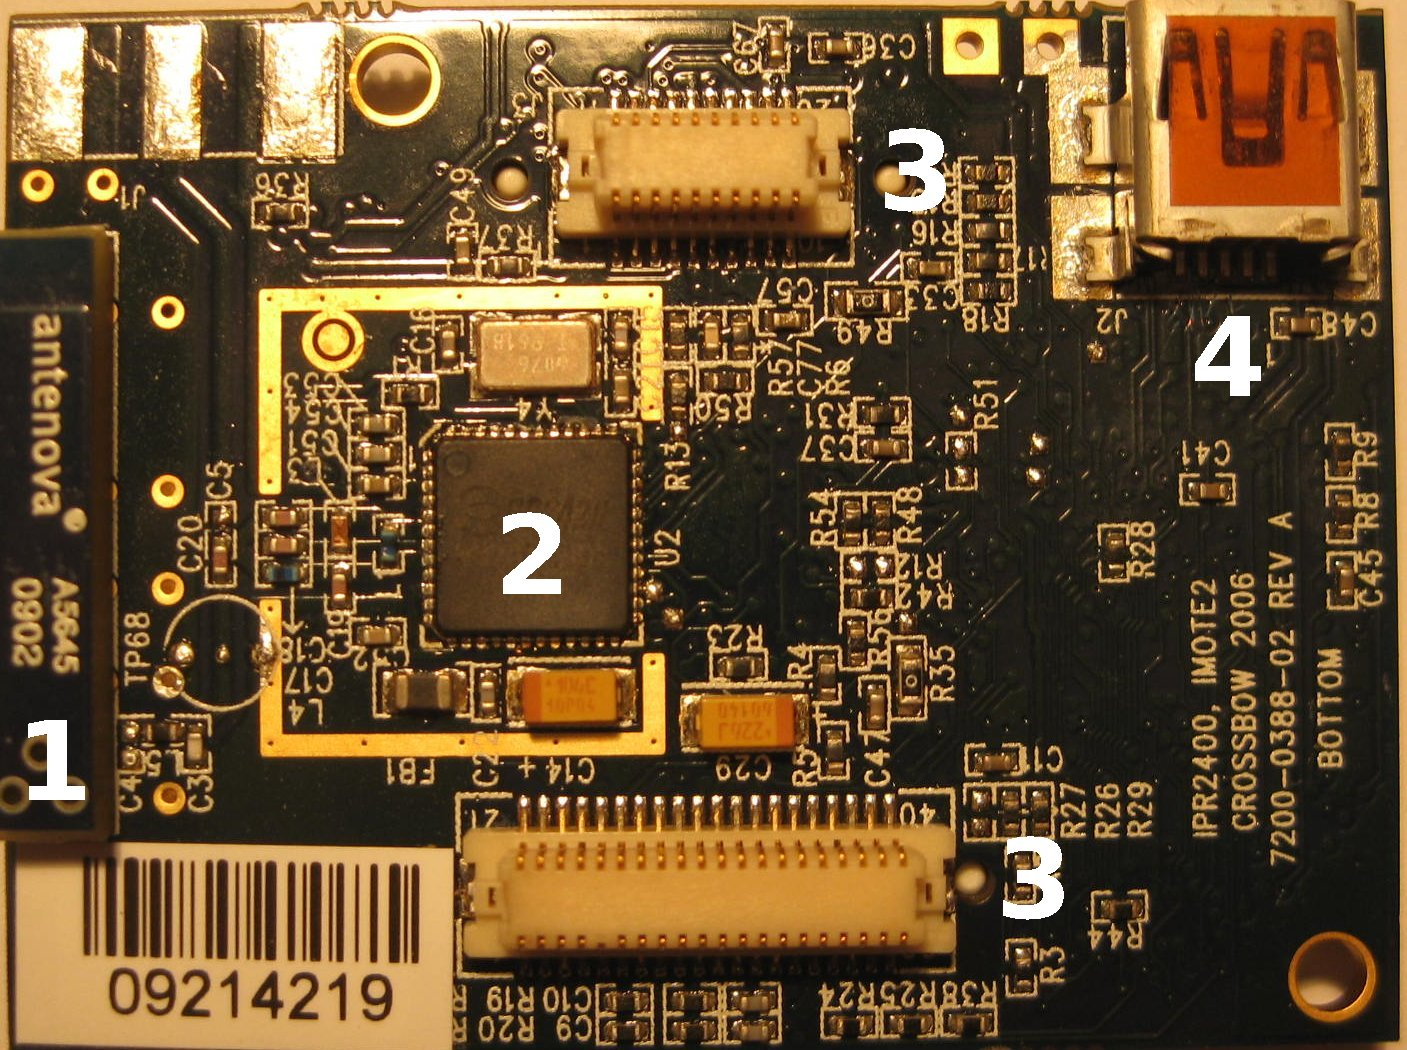
\includegraphics[width=6.5cm]{images/imote_top_cutted2}
    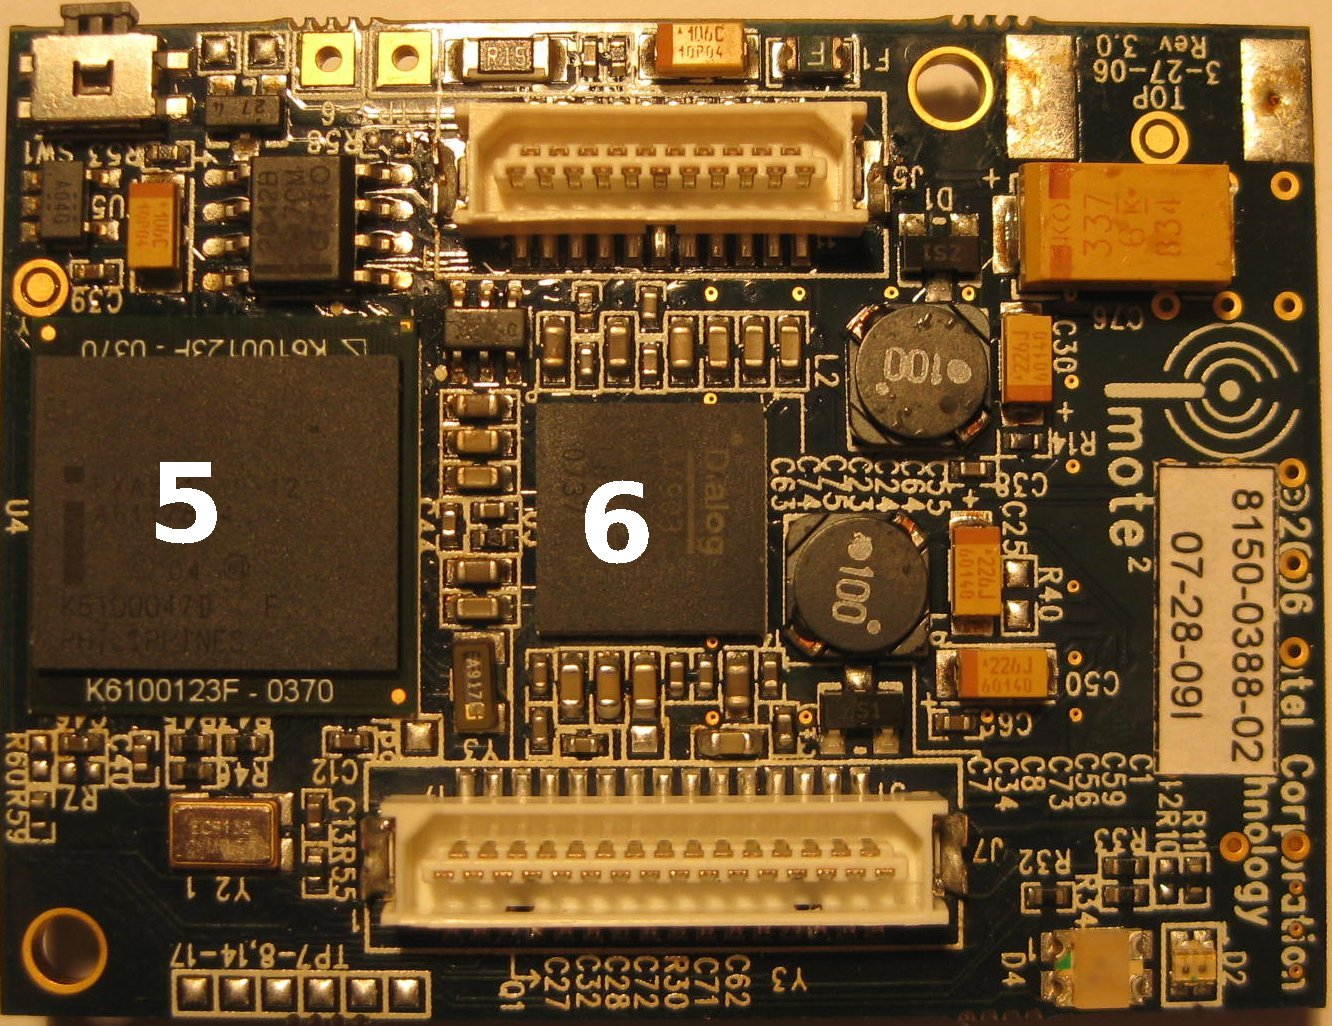
\includegraphics[width=6.5cm]{images/imote_bottom_cutted2}
    \caption{Top side of the Processor Radio Board with antenna (1), the CC2420 (2),
	     the board connectors (3) and the USB connector (4) on the left side
	     and the bottom side with the PXA processor (5) and power management
	     chip (6) on the right}
        \label{fig:imote2top}
  \end{center}
\end{figure}

\section{CC2420 IEEE 802.15.4 Transceiver}
\label{cc2420}
The IEEE 802.15.4 radio used on the Imote2 is a CC2420~\cite{cc2420} from TI (formerly ChipCon).
Configuration and data transfer is done over SPI while some extra signalling
GPIOs are used for interrupts. The hardware also features a FIFO for transmit as
well as for receive. Both FIFOs have a size of 128 bytes which is the maximum
transfer unit in IEEE 802.15.4. Interrupts are generated once a start frame delimiter
(SFD) has been recognized, a full packet has arrived in the FIFO or when a FIFO is
about to reach a specified threshold.

The CC2420 is a full-function device (FFD) and as such can be used as
coordinator or normal node. It uses only the 2.4 GHz band out of the three
available and supports all sixteen channels on this band (channel 11 / 2.405 GHz
to channel 26 / 2.480 GHz). It also supports the highest data rate available
in IEEE 802.15.4 with 250 kbps. Configuration modes for the radio transmission power
are available to either save power or extend range. The CC2420 falls in the
category of packet-based radio. Packet-based radios are implementing parts of
the physical layer already in hardware. This brings the benefit of less software
complexity to drive the chip.

Additional hardware support is available for CRC calculation, data encryption, clear
channel assignment, auto acknowledge, link quality indication and more. Due to
his extensive hardware support this chip is also used in many microcontroller
based systems. It is easy to integrate the SPI interface as well as the GPIO and
interrupt lines into a system and the software support to drive the chip can be
stripped down to a minimum if needed.

The only disadvantage is the lack of support for all frequency bands. The 2.4 GHz
industrial, scientific and medical (ISM) band is already crowded with WiFi
communication, baby monitors, home video streaming solutions and many other
transmitters. Having a chip that would be able to use the other radio bands
would have opened the possibility to switch to a less crowded band and evaluate
the performance in contrast to the 2.4 GHz band.


\chapter{Base System}
This chapter describes the basic software system we are using on the Imote2
platform. Ranging from the bootloader throught the Linux kernel up to the
userland software stack. Our DTN implementation, IBR-DTN, is excluded here as we
describe them in detail in a separate chapter.

\section{Bootstraping}
The Imote2 comes with TinyOS pre-installed. No bootloader or similar mechanism
is installed to allow reflashing of the device. As a last resort there is JTAG
available on the interface board and we used it together with OpenOCD and an
JTAGKeyTiny to bootstrap our linux system. Blob was used as bootloader to load
the kernel image from flash and give the right parameter to boot into the
userland root file system. Detailed steps can be found in the annex.

\section{Linux Kernel}
A recent Linux kernel (2.6.33) is used on the device. The basic support for the
PXA271 and the Imote2 board was already available in this kernel.

\section{CC2420 Driver and ieee802154 stack}

\section{OpenEmbedded base system}


\chapter{IBR-DTN}
\label{ibr-dtn}
\section{IBR-DTN}

IBR-DTN is an implementation of the DTN bundle protocol~\cite{RFC5050}. It is
designed and implemented with efficiency in mind. Efficient memory usage is critical
for use in embedded systems like wireless routers or smartphones. Another design
goal is the interoperability with the DTN2 reference implementation by the Delay
Tolerant Networking Research Group (DTNRG). In contrast to the reference
implementation it can cope with only 4 MByte of memory. That way it can be run
on wireless routers or similar constrained devices.

It features a UDP, TCP and a HTTP convergence layer. All three are targeted at
compliance to the respective internet drafts. The work done for this thesis lays
the groundwork for the forthcoming convergence layer in IBR-DTN. The details and
shortcomings of our work are discussed in chapter~\ref{802154layer}. All these
convergence layers are handled by the Convergence Layer Manager as part of the
modular design of IBR-DTN.

Another module handles the storage of bundles either in memory or on persistent
storage. This allows flexible handling of different kinds of scenarios. With
persistent storage it is for example possible to forward a bundle received earlier
even if the device had a power outage. To know which other nodes are reachable
IBR-DTN offers two mechanisms. The first one is discovery which can be based on
the UDP or TCP convergence layer as well as the IP neighbour discovery draft for
DTN. The second way is to set static routes for the nodes inside the
configuration file of IBR-DTN. This maps the name of a DTN node to its address
and maybe some needed routing. Next to the default routing strategy there is
also an implementation of epidemic routing with bloomfilter.

Once a new node is discovered the bundles stored for it are forwarded immediately.
Some small applications that allow comfortable testing and debugging are also
included in the suite: Dtnping for round trip time measurement as well as simple
bundle send and receive tools.

\section{DTN Convergence Layer}
The role of a convergence layer in DTN is to encapsulate the details of the
transport protocol from the rest of the bundle protocol. If the DTN core is in
need to send out a bundle it uses the \emph{queue} method of the convergence
layer to pass the bundle data and destination node informations to the
convergence layer.

All details about the bundle transmission are handled within the convergence
layer and its helper functions. How complex the convergence layer needs to be
depends on the transport protocol it implements. In general it can be split into
three parts: establishing a connection, transfer the data and closing a
connection.

The receiving path the convergence layer listens for incoming data and up on
complete receive sends the bundle into the DTN core for further processing. All
details about possible packet reassembling or fragmentation are again hidden
from the DTN core by the convergence layer.

\section{Other DTN Implementations}
As briefly mentioned above there are other implementations of the bundle
protocol available. ION~\footnote{https://ion.ocp.ohiou.edu/} is, like IBR-DTN,
a Linux/Unix implementation. DASM~\cite{dasm} is an implementation for Symbian.
DTNLite~\cite{dtnlite} and ContikiDTN~\cite{contikidtn} are written for TinyOS and
Contiki respectively. Those are the ones that are the closest to our work we
have done here. We discuss them in section~\ref{relatedwork}.


\chapter{IEEE 802.15.4 Convergence layer}
\label{802154layer}
\section{Interface with the Linux ieee802154 Stack}

Like the convergence layers for UDP or TCP the job of the IEEE 802.15.4
convergence layer is it to mediate between the Linux kernel provided interface
to the ieee802514 stack and the IBR-DTN core. It has no knowledge about the
bundle protocol or other DTN specific internals but provides only classes and
functions to find a node, address it and transfer the raw data.

The communication between the IEEE 802.15.4 convergence layer of IBR-DTN and the
Linux ieee802154 stack is done over two separate channels. One is used for
signalling and configuration and is handled over the kernel netlink mechanism.
The second is used for the actual data transport and is exposed as standard
socket interface. Listing \ref{lstsocketapi} shows the usage of the socket interface.
As domain AF\_IEEE802154 is used and a struct sockaddr\_ieee802154 fulfills the
need for an adjustment of the addressing scheme as well as the usage of a PAN
ID. The type is the known SOCK\_DGRAM and the default protocol is used. In the
convergence layer we use the socket interface to transmit the data to the actual
peer. The functionlaity is wrapped into a UnicastSocketLOWPAN class.

\begin{lstlisting}[caption= ieee802154 socket interface, label=lstsocketapi]
        int sd;
        struct sockaddr_ieee802154 a;

        sd = socket(PF_IEEE802154, SOCK_DGRAM, 0);

        a.family = AF_IEEE802154;
        a.addr.addr_type = IEEE802154_ADDR_SHORT;
        a.addr.pan_id = 0x0780;

	a.addr.short_addr = 0x0001;
	bind(sd, (struct sockaddr *)&a, sizeof(a));

        a.addr.short_addr = 0x8001;
	connect(sd, (struct sockaddr *)&a, sizeof(a));
\end{lstlisting}

Over netlink it is possible to send different commands and a set attributes to the
ieee802154 stack. The attributes contain among others informations about the
address of the interface, its index, PAN ID, channel and more. The commands
allow to get and set the different attributes, trigger a association, request a
scan and others. The given functionality is used to implement the basic
utilities for configuration as well as a PAN coordinator bundled together in
the lowpan-tools package. In IBR-DTN we only use a small subset of this
functionality. We use the given interface name to ask for its short address when
binding to the socket to receive incoming data. In the future we could also ask for
the PAN ID and the hardware address to be more flexible.

For the basic network setup we rely on the lowpan-tools utilities. With
\emph{izcoordinator} we set up a PAN coordinator on one
node while we use \emph{iz} to associate to this PAN from the other node. The PAN ID is
given to both tools on the commandline and the coordinator hands the
associating node a short address. With this basic configuration, which can
somewhat be compared to a DHCP server and client, we start dtnd and are ready to
transmit and receive bundles.

\section{Configuration}

To make IBR-DTN work correctly with our IEEE 802.15.4 hardware we need to configure
it and teach it about the interface name it has to use as well as that we are
looking for a zigbee connection. Lowpan is just the internal name for the
IEEE 802.15.4 convergence layer inside IBR-DTN. The PAN ID needs to be filled into the
port configuration option. Filled in values need to be in decimal notation.

Listing \ref{lstconfig} also shows the configuration for static routes to other
nodes.

\begin{lstlisting}[caption= dtnd example configuration, label=lstconfig]
cal_uri = dtn://1.dtn
net_interfaces = lan0
net_lan0_type = lowpan
net_lan0_interface = wpan0
net_lan0_port = 1920		#0x780

routing = default

# Static connections
static1_address = 32769         #0x8001
static1_port = 1920		#0x780
static1_uri = dtn://2.dtn
static1_proto = zigbee
\end{lstlisting}

\section{Addressing}

The specification for Low-Rate Wireless Personal Area Networks specifies two
types of addresses. All devices have an unique 64 bit extended address.
Additional they can have a 16 bit short address that can be different depending
on the PAN. The short address is supplied by the PAN coordinator. for now we
only support the short address type in IBR-DTN. Support for extended addresses
are planned for the future. As well as the discovery of other nodes over a
mbroadcast mechanism. Such a braodcast could be done by sending it to the 0xffff
address with the correct PAN ID to reach all nodes within the PAN or with 0xffff
as PAN ID to reach all nodes in range.

\section{Fragmentation}

The maximal packet size in IEEE 802.15.4 is about 128 byte. Deducting the header
and other needed data we can transport about 115 byte of actual payload in a
packet. This payload size is way smaller to what other IBR-DTN convergence
layers have used before. They have been build around the IP/TCP/UDP family which
normally has a maximal transfer size of 1500 byte.

The header size of the bundle protocol is not fixed but variable depending on
the transported data and enabled options. It is as well possible that the header
size is greater then the 115 byte payload we could offer with IEEE 802.15.4. The
draft \cite{tcp-clayer-draft} for a TCP convergence layer protocol could help here as it
defines a data transmission divided into several segments. Even the bundle
header could be split into several segments this way and build together on the
receiving side.

\section{Related Work}

While DTN is getting more popular for research there are only a few research
projects then combine DTN with sensor network technologies like IEEE 802.15.4.
That is not surprising if one keeps in mind that the DTN architecture is is
complex and memory as well as bandwidth consuming. Both resources that are scare
on sensor network platforms.

Two projects are aiming to explore this area of research. One of them is the
TinyOS based DTNLite \cite{dtnlite}. It is loosely based on the DTN overlay
architecture. To deliver custody transfer over the overlay they use techniques
like asynchronous message delivery. The concept is targeted at data collection
applications which need to reach a central station for the collection over the
network. The applications must be written or re-written to be DTNLite aware.

ContikiDTN \cite{contikidtn} is, like DTNLite, written for a special purpose embedded operating
system in this case Contiki \footnote{http://www.sics.se/contiki/}. While
DTNLite only aims to work with other DTNLite installations Contiki DTN aims for
ContikiDTN is tied to only work with a TCP convergence layer. It was a design
choice that no other convergence layer can be plugged in. This restriction goes
down to the used µIP component of Contiki which offers the used protosockets
only work with TCP.

Both implementations have not been suitable for our work as they are either not
standard compliant or have a design restriction to only TCP. Furthermore both
are designed around a special purpose operating system while our aim was to work
on the general purpose operating system Linux.


\chapter{Evaluation}
To verify our work on the convergence layer as well as compare it to other and
find potential bottlenecks we evaluated out work under different test cases.
Comparing the data throughput and packetloss for raw IEEE 802.15.4 against DTN
as an additional layer. Distance measurement as well as Round Trip Time
measurement was also done.

\section{Throughput}
For the real payload data throughput we measured the payload data the receiving
nodes could receive over time. We did the measurement for raw IEEE 802.154 and
DTN traffic separately. For both test cases we send packages with the maximum
payload from one node to another as fast as the system allowed. The maximum
payload length for IEEE 802.15.4 packets have been 115 byte and for DTN 40 byte.

During this tests a problem in the lower layers of the system showed up. It is
still unclear if it is a driver or problem with the ieee802154 stack. The
problem showed up when we tried to send the packets as fast as possible over the
socket interface. After some packets the kernel part got stuck and stopped
transmitting while still accepting data over the socket. The kernel log output
showed a unbalanced IRQ as potential reason for the problem. Time did not allow
to go to the ground of this problem and fix it probably so we went with a delay
in the test application to circumvent this. We added a 100ms delay in the send
routine and the lookup went away. It was the smallest value we could still
reliable send data with. Obviously such a big delay has a negative impact on the
throughput, but without it no measurement would have been possible at all.

Figure FIXME shows the data we collected with different distances between the
nodes.

\section{Packetloss}
Throughput alone is of course nothing that tells us much about how reliable a
connection is. Therefor we also measured the packet loss while doing the
throughput measurements. Inside the packet payload a sequence number was encoded
and during a post process the lost packet rate was calculated. No retransmission
was done on the lower layers to avoid even more negative impact on the
throughput and wrong statistics in this test.

Figure FIXME shows the constant raise of the lost packet rate over the distance
we did our measurements.

\section{Distance}
The Imote2 has no connector for an external antenna but an on-board antenna
only. To get an understanding what use cases this antenna, and therefor the
whole board, could cover we combined our measurements with a distance
measurement. To decide if a distance is still usable enough we used the
packetloss as quality indicator. All distances which showed a packetloss above
50 percent are rated as unusable. During our measurements such a high packetloss
was shown for all distances higher then 33m.

\section{DTN Round Trip Time}
The last testcase was the round trip time of a DTN bundle. We used the
\emph{dtnping} utility to send out a bundle, receive the answer and calculate
the round trip time. Bundles are send to the \emph{echo} application of the
receiving node. In our case this is directly the DTN daemon. The default payload
size of a ping bundle was to big to our limited payload size on the IEEE
802.15.4 convergence layer. We reduced the payload to 1 byte and used it for all
tests. Table \ref{dtnrtt} shows the results of the measurement in milliseconds. We
had 10 different scenarios for this test case and did five measurements for each.
The first eight are the same we used for our throughput and packetloss test cases.
We added two more scenarios to compare it against our usual test environment. The
local scenario did send bundles over the UDP convergence layer on the loopback
interface of our X86 workstation while the UDP scenario did send the bundles
through the UDP convergence layer over an 1 Gbit Ethernet link to another
machine.

\begin{table}
\begin{tabular}{l*{9}{c}r}
    & 0m & 1m & 5m & 10m & 15m & 20m & 25m & 30m & local & UDP \\
\hline
Min & 656.14 & 651.11 & 664.25 & 645.27 & 659.29 & 651.40 & 653.66 & 677.29 & 38.31 & 40.90 \\
Mean & 676.17 & 662.38 & 674.85 & 674.85 & 676.46 & 672.03 & 672.47 & 686.60 & 38.87 & 41.26 \\
Max & 693.14 & 678.49 & 684.96 & 685.11 & 695.76 & 684.22 & 687.26 & 693.64 & 39.41 & 41.56 \\
\end{tabular}
\caption{ DTN Round Trip Time measurement results}
\label{dtnrtt}
\end{table}


\chapter{Conclusion}
This thesis showed that it is possible to use a standard compliant DTN
implementation on top of a IEEE 802.15.4 network. That was not obvious from the
beginning and can be seen as a success. We found and corrected problems in the
driver and Linux kernel stack for IEEE 802.15.4 and wrote a convergence layer to
adapt IBR-DTN to it. The evaluation was used for performance measurement and
showed us the actual performance as well as areas for improvements.

Being the first project implementing standard compliant DTN over a IEEE 802.15.4
link allowed us to proof that both technologies can work together. This opens up
a complete new field of research. Using delay tolerant networking in low-power
wireless sensor networks allows multi-hop transmission of sensor data following
the store and forward principle of DTN. Nodes must no longer be in range to
transmit data but can send it out to all other nodes in range which will forward
the data until they reach the destination. The win is a greater flexibility for
sensor node placement and moving sensors.

\section{Future Work}
The new convergence layer supports sending and receiving for bundles up to a
payload of 40 bytes. That is the biggest limitation of the current work. To
improve this situation different approaches can be taken. One of the newest
additions in IBR-DTN is header compression. This technique makes it possible to
shrink the header by using numerical addresses and avoid the dictionary to be
transmitted. Given that the current ratio in a bundle over IEEE 802.15.4 is two
thirds for the header and only one third for the actual payload that would indeed
improve the situation. To solve the problem for larger bundles a fragmentation
within the convergence layer could be used to split the bundles into smaller
chunks, transmit and then reassemble them within the convergence layer on the
receiving side. Such a mechanism is already described in the TCP convergence
layer draft~\cite{tcp-clayer-draft} and implemented in IBR-DTN. In the future
work this could be adapted to the IEEE 802.15.4 convergence layer to fully
solve the problem of the restricted payload length.

The evaluation also revealed some initial performance statistics which can be
used to improve the current implementation. One of the most interesting points
is that the raw IEEE 802.15.4 data throughput performance, without any DTN
involved, is already way below the theoretical maximum of 250 kbps. With only
4600 bps it reaches only 1.8 percent of the theoretical maximum. Partly this
comes from a delay added in the test application to allow a reliable test
environment still this explains not everything. Future research on this topic
should allow to pinpoint performance bottlenecks in the driver and Linux stack
as well as in IBR-DTN.


\addcontentsline{toc}{chapter}{Literature}
\bibliographystyle{unsrt}
\bibliography{thesis}

\begin{appendix}

\chapter{Flashing with OpenOCD}
\label{annexopenocd}
\parindent=0pt                   % erzeugt bei einem Absatz eine
\parskip=6pt plus 3pt            % Leerzeile (kein Einruecken)

Use OpenOCD to do the initial blob install:

The Imote2 is shipped with TinyOS by default. There is no bootloader installed
that would allow you to flash another OS so the only way to get it bootstrapped
was to use the JTAG interface.

We used OpenOCD for this task. Make sure you have at least OpenOCD version 0.4.0
and libftdi version 0.17 installed.

The OS we are going to install consists of the major parts. The bootloader blob, the
Linux kernel and a root file system with the userland software components. While
we are preparing the kernel and the root filesystem ourself we use a
precompiled version of the blob bootloader from:
http://sourceforge.net/projects/imote2-linux/files/

The used JTAG adapter is a JTAGkey Tiny from Amontec. OpenOCD already offers
configurations for the JTAG adapter as well as the Imote2 board. Starting
OpenOCD as following uses the right configuration files:

\begin{verbatim}
sudo openocd -f /usr/share/openocd/scripts/interface/jtagkey.cfg -f \\
/usr/share/openocd/scripts/board/crossbow\_tech\_imote2.cfg
\end{verbatim}

Now you can connect to the OpenOCD telnet interface on port 4444 with:

\begin{verbatim}
telnet localhost 4444
\end{verbatim}

First we need to make sure that the Imote2 is halted. In this state we are at PC
0 and no code got executed so far. Afterwards we disable the flash protection and
erase the complete flash. The last three steps are writing the bootloader, the
Linux kernel and the root filesystem at the given offsets into the flash. The last
step will take a long time as it writes 30 Mbyte into the flash.

\begin{verbatim}
# reset halt
# flash protect 0 0 last off
# flash erase_sector 0 0 258
# flash write_image blob-im2
# flash write_image 2.6.34-rc2-zImage 0x00040000 bin
# flash write_image console-image-imote2.jffs2 0x00240000 bin
\end{verbatim}

\chapter{OpenEmbedded}
\label{annexoe}

OpenEmbedded \footnote{http://www.openembedded.org/} is a build framework for
embedded Linux. It provides the meta-data which incorporates the knowledge how
to fetch, build, install, package and more for over 5000 Open Source projects.

Adding support for the Imote2 hardware to it did only required us to add a
\emph{machine configuration} which describes the hardware and let OpenEmbedded
know about it. Below is this machine configuration we added:

\begin{verbatim}
#@TYPE: Machine
#@Name: Crossbow iMote2
#@DESCRIPTION: Machine configuration for Crossbow iMote 2
TARGET_ARCH = "arm"
PREFERRED_PROVIDER_virtual/kernel = "linux"
PACKAGE_EXTRA_ARCHS = " iwmmxt"
KERNEL_IMAGETYPE = "zImage"
IMAGE_FSTYPE += "jffs2"
EXTRA_IMAGECMD_jffs2 = "--l --pad=0x01DC0000 --eraseblock=0x20000"
CMDLINE="root=/dev/mtdblock2 rootfstype=jffs2 console=ttyS2,115200"
SERIAL_CONSOLE = "115200 ttyS2"
require conf/machine/include/tune-xscale.inc
ROOT_FLASH_SIZE ?= "30"
MACHINE_FEATURES = "kernel26 usbgadget alsa iwmmxt"
\end{verbatim}

We also added the needed meta-data for the Linux kernel used on our Imote2 and
the build description for IBR-DTN. In a final step we put all this together in
an image that could be build with the \emph{bitbake} application. BitBake uses
the meta-data provided by OpenEmbedded to actually build the software and the
resulting firmware and kernel images.

After this we were able to create our complete firmware image by just executing
BitBake like this:

\begin{verbatim}
bitbake imote2-image
\end{verbatim}

All our changes are already included in the OpenEmbedded source code repository
and could be used from there. The latest git revision we used for our work was
6fc1c96131d4c4afabe815148f8e55656fb7f402. If any newer version have problems it
is possible to revert back to this known good revision for future work.


\end{appendix}

\end{document}
